% Task 1
\documentclass[12pt,a4paper,english]{extarticle}
\usepackage[T1]{fontenc}
\usepackage[utf8]{inputenc}
\usepackage{fourier}
\usepackage{geometry}
\geometry{verbose,tmargin=2.2cm,bmargin=2cm,lmargin=2.2cm,rmargin=2cm}
\usepackage{float}
\usepackage{textcomp}
\usepackage{amsmath}
\usepackage{stackrel}
\usepackage{graphicx}
\usepackage{esint}
\usepackage{tikz}
\usepackage{array}
\usepackage{multirow}
\usetikzlibrary{matrix,calc}

\makeatletter

\providecommand{\tabularnewline}{\\}

\usepackage{fancyhdr}
\usepackage{lscape}
\usepackage{amssymb}
\pagestyle{fancy}
\lhead{Electronica III - 22.13}
\chead{TPL3}
\rhead{ITBA}
\renewcommand{\headrulewidth}{1pt}
\renewcommand{\footrulewidth}{1pt}

\makeatother

\usepackage[english]{babel}

\usepackage{tikz}
\usetikzlibrary{matrix,calc}

%isolated term
%#1 - Optional. Space between node and grouping line. Default=0
%#2 - node
%#3 - filling color
\newcommand{\implicantsol}[3][0]{
    \draw[rounded corners=3pt, fill=#3, opacity=0.3] ($(#2.north west)+(135:#1)$) rectangle ($(#2.south east)+(-45:#1)$);
    }


%internal group
%#1 - Optional. Space between node and grouping line. Default=0
%#2 - top left node
%#3 - bottom right node
%#4 - filling color
\newcommand{\implicant}[4][0]{
    \draw[rounded corners=3pt, fill=#4, opacity=0.3] ($(#2.north west)+(135:#1)$) rectangle ($(#3.south east)+(-45:#1)$);
    }

%group lateral borders
%#1 - Optional. Space between node and grouping line. Default=0
%#2 - top left node
%#3 - bottom right node
%#4 - filling color
\newcommand{\implicantcostats}[4][0]{
    \draw[rounded corners=3pt, fill=#4, opacity=0.3] ($(rf.east |- #2.north)+(90:#1)$)-| ($(#2.east)+(0:#1)$) |- ($(rf.east |- #3.south)+(-90:#1)$);
    \draw[rounded corners=3pt, fill=#4, opacity=0.3] ($(cf.west |- #2.north)+(90:#1)$) -| ($(#3.west)+(180:#1)$) |- ($(cf.west |- #3.south)+(-90:#1)$);
}

%group top-bottom borders
%#1 - Optional. Space between node and grouping line. Default=0
%#2 - top left node
%#3 - bottom right node
%#4 - filling color
\newcommand{\implicantdaltbaix}[4][0]{
    \draw[rounded corners=3pt, fill=#4, opacity=0.3] ($(cf.south -| #2.west)+(180:#1)$) |- ($(#2.south)+(-90:#1)$) -| ($(cf.south -| #3.east)+(0:#1)$);
    \draw[rounded corners=3pt, fill=#4, opacity=0.3] ($(rf.north -| #2.west)+(180:#1)$) |- ($(#3.north)+(90:#1)$) -| ($(rf.north -| #3.east)+(0:#1)$);
}

%group corners
%#1 - Optional. Space between node and grouping line. Default=0
%#2 - filling color
\newcommand{\implicantcantons}[2][0]{
    \draw[rounded corners=3pt, opacity=.3] ($(rf.east |- 0.south)+(-90:#1)$) -| ($(0.east |- cf.south)+(0:#1)$);
    \draw[rounded corners=3pt, opacity=.3] ($(rf.east |- 8.north)+(90:#1)$) -| ($(8.east |- rf.north)+(0:#1)$);
    \draw[rounded corners=3pt, opacity=.3] ($(cf.west |- 2.south)+(-90:#1)$) -| ($(2.west |- cf.south)+(180:#1)$);
    \draw[rounded corners=3pt, opacity=.3] ($(cf.west |- 10.north)+(90:#1)$) -| ($(10.west |- rf.north)+(180:#1)$);
    \fill[rounded corners=3pt, fill=#2, opacity=.3] ($(rf.east |- 0.south)+(-90:#1)$) -|  ($(0.east |- cf.south)+(0:#1)$) [sharp corners] ($(rf.east |- 0.south)+(-90:#1)$) |-  ($(0.east |- cf.south)+(0:#1)$) ;
    \fill[rounded corners=3pt, fill=#2, opacity=.3] ($(rf.east |- 8.north)+(90:#1)$) -| ($(8.east |- rf.north)+(0:#1)$) [sharp corners] ($(rf.east |- 8.north)+(90:#1)$) |- ($(8.east |- rf.north)+(0:#1)$) ;
    \fill[rounded corners=3pt, fill=#2, opacity=.3] ($(cf.west |- 2.south)+(-90:#1)$) -| ($(2.west |- cf.south)+(180:#1)$) [sharp corners]($(cf.west |- 2.south)+(-90:#1)$) |- ($(2.west |- cf.south)+(180:#1)$) ;
    \fill[rounded corners=3pt, fill=#2, opacity=.3] ($(cf.west |- 10.north)+(90:#1)$) -| ($(10.west |- rf.north)+(180:#1)$) [sharp corners] ($(cf.west |- 10.north)+(90:#1)$) |- ($(10.west |- rf.north)+(180:#1)$) ;
}

%Empty Karnaugh map 4x4
\newenvironment{Karnaugh}%
{
\begin{tikzpicture}[baseline=(current bounding box.north),scale=0.8]
\draw (0,0) grid (4,4);
\draw (0,4) -- node [pos=0.7,above right,anchor=south west] {y2y1} node [pos=0.7,below left,anchor=north east] {SI} ++(135:1);
%
\matrix (mapa) [matrix of nodes,
        column sep={0.8cm,between origins},
        row sep={0.8cm,between origins},
        every node/.style={minimum size=0.3mm},
        anchor=8.center,
        ampersand replacement=\&] at (0.5,0.5)
{
                       \& |(c00)| 00         \& |(c01)| 01         \& |(c11)| 11         \& |(c10)| 10         \& |(cf)| \phantom{00} \\
|(r00)| 00             \& |(0)|  \phantom{0} \& |(1)|  \phantom{0} \& |(3)|  \phantom{0} \& |(2)|  \phantom{0} \&                     \\
|(r01)| 01             \& |(4)|  \phantom{0} \& |(5)|  \phantom{0} \& |(7)|  \phantom{0} \& |(6)|  \phantom{0} \&                     \\
|(r11)| 11             \& |(12)| \phantom{0} \& |(13)| \phantom{0} \& |(15)| \phantom{0} \& |(14)| \phantom{0} \&                     \\
|(r10)| 10             \& |(8)|  \phantom{0} \& |(9)|  \phantom{0} \& |(11)| \phantom{0} \& |(10)| \phantom{0} \&                     \\
|(rf) | \phantom{00}   \&                    \&                    \&                    \&                    \&                     \\
};
}%
{
\end{tikzpicture}
}

%Empty Karnaugh map 2x4
\newenvironment{Karnaughvuit}%
{
\begin{tikzpicture}[baseline=(current bounding box.north),scale=0.8]
\draw (0,0) grid (4,2);
\draw (0,2) -- node [pos=0.7,above right,anchor=south west] {bc} node [pos=0.7,below left,anchor=north east] {a} ++(135:1);
%
\matrix (mapa) [matrix of nodes,
        column sep={0.8cm,between origins},
        row sep={0.8cm,between origins},
        every node/.style={minimum size=0.3mm},
        anchor=4.center,
        ampersand replacement=\&] at (0.5,0.5)
{
                      \& |(c00)| 00         \& |(c01)| 01         \& |(c11)| 11         \& |(c10)| 10         \& |(cf)| \phantom{00} \\
|(r00)| 0             \& |(0)|  \phantom{0} \& |(1)|  \phantom{0} \& |(3)|  \phantom{0} \& |(2)|  \phantom{0} \&                     \\
|(r01)| 1             \& |(4)|  \phantom{0} \& |(5)|  \phantom{0} \& |(7)|  \phantom{0} \& |(6)|  \phantom{0} \&                     \\
|(rf) | \phantom{00}  \&                    \&                    \&                    \&                    \&                     \\
};
}%
{
\end{tikzpicture}
}

%Empty Karnaugh map 2x2
\newenvironment{Karnaughquatre}%
{
\begin{tikzpicture}[baseline=(current bounding box.north),scale=0.8]
\draw (0,0) grid (2,2);
\draw (0,2) -- node [pos=0.7,above right,anchor=south west] {b} node [pos=0.7,below left,anchor=north east] {a} ++(135:1);
%
\matrix (mapa) [matrix of nodes,
        column sep={0.8cm,between origins},
        row sep={0.8cm,between origins},
        every node/.style={minimum size=0.3mm},
        anchor=2.center,
        ampersand replacement=\&] at (0.5,0.5)
{
          \& |(c00)| 0          \& |(c01)| 1  \\
|(r00)| 0 \& |(0)|  \phantom{0} \& |(1)|  \phantom{0} \\
|(r01)| 1 \& |(2)|  \phantom{0} \& |(3)|  \phantom{0} \\
};
}%
{
\end{tikzpicture}
}

%Defines 8 or 16 values (0,1,X)
\newcommand{\contingut}[1]{%
\foreach \x [count=\xi from 0]  in {#1}
     \path (\xi) node {\x};
}

%Places 1 in listed positions
\newcommand{\minterms}[1]{%
    \foreach \x in {#1}
        \path (\x) node {1};
}

%Places 0 in listed positions
\newcommand{\maxterms}[1]{%
    \foreach \x in {#1}
        \path (\x) node {0};
}

%Places X in listed positions
\newcommand{\indeterminats}[1]{%
    \foreach \x in {#1}
        \path (\x) node {X};
}

% \begin{document}
%     \begin{Karnaugh}
%         \contingut{0,0,0,0,0,0,0,0,0,0,0,0,0,0,0,0}
%        \implicant{0}{2}{red}
%        \implicant{5}{15}{purple}
%        \implicantdaltbaix[3pt]{3}{10}{blue}
%     \implicantcantons[2pt]{orange}
%        \implicantcostats{4}{14}{green}
%     \end{Karnaugh}
%     %
%     \begin{Karnaughvuit}
%        \minterms{3,4}
%         \maxterms{0,1,6,7}
%        \indeterminats{2,5}
%        \implicant{3}{2}{green}
%        \implicant{4}{5}{}
%     \end{Karnaughvuit}
%     %
%     \begin{Karnaughquatre}
%         \minterms{1,2}
%        \maxterms{0,3}
%        \implicantsol{1}{green}
%        \implicantsol{2}{red}
%     \end{Karnaughquatre}

% \end{document}
\begin{document}
\providecommand{\tabularnewline}{\\}
\section*{Task 1}

In this section, a state machine will be 
developed for controlling the switching
on and off of two pumps, to fill a tank.
The are controlled by two sensors from 
the upper part of the tank (S) and the 
lower part of the tank (I). The actions
to take are as follows:

\begin{itemize}
    \item Tank full: S = I = 1 - Pumps OFF
    \item Tank empty: S = I = 0 - Pumps ON
    \item Half full tank: S = 0 \& I = 1 - Pumps alternate 
\end{itemize}

With this in mind, a Moore machine is 
developed as follows.

\begin{figure}[H]
    \begin{centering}
    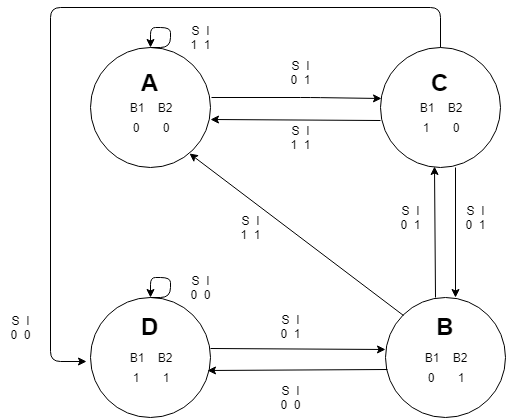
\includegraphics[width=0.8\textwidth]{Graficos1/1a_fsm.png}
    \par\end{centering}
    \caption{Moore state machine diagram}
\end{figure}

Using two bits to asign the states, a table 
of transitions is made, as shown below.

\begin{figure}[H]
\begin{centering}
\begin{tabular}{|c|c|c|c|c|c||c|c|}
    \hline 
    \multicolumn{2}{|c|}{Estado Actual} & \multicolumn{4}{c||}{Estado Siguiente} & \multicolumn{2}{c|}{Salidas}\tabularnewline
    \hline 
    \hline 
    \multirow{2}{*}{} & \multirow{2}{*}{y2 - y1} & \multicolumn{4}{c||}{S - I} & \multirow{2}{*}{B1} & \multirow{2}{*}{B2}\tabularnewline
    \cline{3-6} 
     &  & 00 & 01 & 10 & 11 &  & \tabularnewline
    \hline 
    A & 00 & X & C & X & A & 0 & 0\tabularnewline
    \hline 
    B & 01 & D & C & X & A & 0 & 1\tabularnewline
    \hline 
    C & 10 & D & B & X & A & 1 & 0\tabularnewline
    \hline 
    D & 11 & D & B & X & X & 1 & 1\tabularnewline
    \hline 
    \end{tabular}
    \caption{Moore state machine - Transitions}
\end{centering}
\end{figure}

\newpage

From the table, using Karnaugh's maps the 
functions for the state variables and the 
two pumps outputs are made as shown below.

\begin{center}
\begin{Karnaugh}
     \contingut{X,1,1,1,1,1,0,0,X,X,X,X,0,0,0,X}    
     \implicant{0}{5}{red}
     \implicantdaltbaix[3pt]{0}{10}{blue}
\end{Karnaugh}
\begin{Karnaugh}
    \contingut{X,1,1,1,1,1,0,0,X,X,X,X,0,0,0,X}       
    \implicant{3}{6}{red}
    \implicantdaltbaix[3pt]{0}{10}{blue}
\end{Karnaugh}
\end{center}

Where from the left table $Y_2 = \overline{I} + \overline{S} \cdot \overline{y_2}$, 
and from the right $Y_1 = \overline{I} + \overline{S} \cdot y_2$. And for
the outputs, $B_1 = y_2$ and $B_2 = y_1$.  
Finally, the state machine is implemented using 
D Flip Flops:

\begin{figure}[H]
    \begin{centering}
    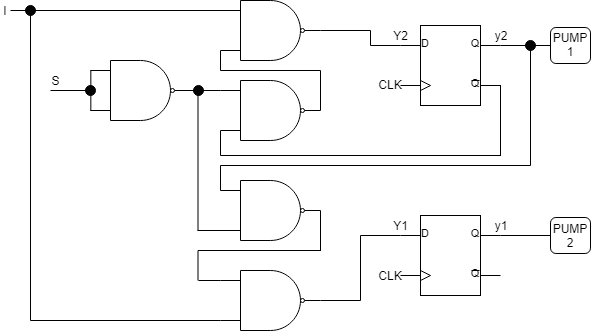
\includegraphics[width=0.7\textwidth]{Graficos1/1a_Compuertas_Moore.png}
    \par\end{centering}
    \caption{Moore state machine - Circuit implementation}
\end{figure}

On the other side, the same system is implemented 
now using a Mealy state machine, as shown below.

\begin{figure}[H]
    \begin{centering}
    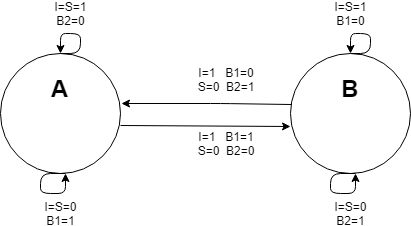
\includegraphics[width=0.7\textwidth]{Graficos1/1b_fsm.png}
    \par\end{centering}
    \caption{Mealy state machine diagram}
\end{figure}

Notice that the direct connection between the 
input and the pumps outputs reduces the number 
of states from four to two, in comparison with 
the Moore machine.
Using one bit for the states, a table of transitions
is made as follows.

\begin{figure}[H]
\begin{centering}
\begin{tabular}{|c|c|c|c|c|c||c|c|c|c|}
    \hline 
    \multicolumn{2}{|c|}{Estado Actual} & \multicolumn{4}{c||}{Estado Siguiente} & \multicolumn{4}{c|}{Salidas}\tabularnewline
    \hline 
    \hline 
    \multirow{3}{*}{} & \multirow{3}{*}{y} & \multicolumn{4}{c||}{S - I} & \multicolumn{4}{c|}{S - I}\tabularnewline
    \cline{3-10} 
     &  & 00 & 01 & 10 & 11 & 00 & 01 & 10 & 11\tabularnewline
    \cline{3-10} 
     &  & \multicolumn{4}{c||}{y} & B1 - B2 & B1 - B2 & B1 - B2 & B1 - B2\tabularnewline
    \hline 
    A & 0 & A & B & A & X & 11 & 10 & XX & 00\tabularnewline
    \hline 
    B & 1 & B & A & B & X & 11 & 01 & XX & 00\tabularnewline
    \hline 
    \end{tabular}
    \caption{Mealy state machine - Transitions}
\end{centering}
\end{figure}

Using again Karnaugh's maps, the functions for
the state variable and the two pumps outputs are
made as shown below.

\begin{center}
     \begin{Karnaughvuit}
        \minterms{1,4,7}
         \maxterms{0,3,5}
        \indeterminats{2,6}
        \implicantsol{1}{red}
        \implicant{7}{6}{green}
        \implicantcostats{4}{6}{blue}
     \end{Karnaughvuit}
     \begin{Karnaughvuit}
        \minterms{0,1,4}
         \maxterms{3,5,7}
        \indeterminats{2,6}
        \implicant{0}{1}{red}
        \implicant{0}{4}{green}
     \end{Karnaughvuit}
     \begin{Karnaughvuit}
        \minterms{0,4,5}
         \maxterms{1,3,7}
        \indeterminats{2,6}
        \implicant{0}{4}{red}
        \implicant{4}{5}{green}
     \end{Karnaughvuit}
\end{center}
Where from the left table $Y = \overline{y} \cdot \overline{S} \cdot I + y \cdot \overline{I} + y \cdot S$. 
From the center table $B_1 = \overline{y} \cdot \overline{S} + \overline{S} \cdot \overline{I}$, and from the 
right table $B_2 = \overline{S} \cdot \overline{I} + y \cdot \overline{S}$.
Finally, the state machine is implemented using
one D Flip Flop.

\begin{figure}[H]
    \begin{centering}
    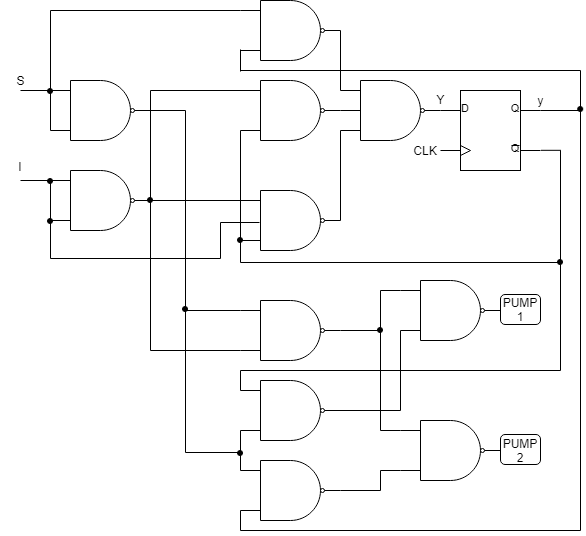
\includegraphics[width=0.7\textwidth]{Graficos1/1b_Compuertas_Mealy.png}
    \par\end{centering}
    \caption{Mealy state machine - Circuit implementation}
\end{figure}

\end{document}